\documentclass[a4paper]{article}

%% Language and font encodings
\usepackage[english]{babel}
\usepackage[utf8x]{inputenc}
\usepackage[T1]{fontenc}

%% Sets page size and margins
\usepackage[a4paper,top=3cm,bottom=2cm,left=3cm,right=3cm,marginparwidth=1.75cm]{geometry}

%% Useful packages
\usepackage{amsmath}
\usepackage{graphicx}
\usepackage[colorinlistoftodos]{todonotes}
\usepackage[colorlinks=true, allcolors=blue]{hyperref}
\usepackage{algorithm2e}
\usepackage{hyperref}
\usepackage{listings}
\usepackage{pgfplots}
\pgfplotsset{compat=1.14}

\setlength{\parindent}{0pt}


\title{Applications of Data Analysis 2018\\Excercise 3}
\author{Timo Heinonen\\509445\\tijuhe@utu.fi}

\begin{document}
\maketitle

\section{Description of the problem}
The goal of this data analysis task was to predict the severity of pain experienced by subjects. The data set contained 5 measurements, heart rate (hr), respitory rate (rrpm), galvanic skin response (gsr), muscle activation of corrugator supercilii (rmscorr) and muscle activation of orbicularis oculi (rmsorb). The subjects reported the intensity of the experienced pain on a scale from one to three.\\

The data set contained 11948 rows from 29 different subjects. Each subject had had 4 test sessions which contained multiple measurements.\\

The response to pain might differ from subject to subject. That's why the data was to be standardized per subject with z-score, as opposed a single standardization. I compared the standardization methods and the resulting C-indices are reported below.\\

I used k-fold cross-validation where each fold contained data from a single subject. Neighbors for each measurement entry were calculated and the majority class of the pain intensity of the neighbors was used as the prediction. C-index was used to measure the model performance.

\section{Algorithm}

\begin{algorithm}[H]
 \KwData{painsignals.csv}
 \KwResult{C-index values for predictions of attributes c-total, cd and pb}
 
 \vspace*{0,5cm}

 Standardize each subject's measurements with z-score\\
 Divide data into \emph{folds} that contain measurements from only one subject\\
 \BlankLine
 \For{\emph{each} fold}{
 	\emph{test\_set} $\leftarrow$ \emph{fold}\\
 	\emph{training\_set} $\leftarrow$ \{ All data $\backslash$ \emph{test\_set} \}\\
    \BlankLine
   	\emph{test\_features} $\leftarrow$ values of hr,rrpm,gsr,rmscorr,rmsorb in \emph{test\_set}\\
    \emph{training\_features} $\leftarrow$ values of hr,rrpm,gsr,rmscorr,rmsorb in \emph{training\_set}\\
    \BlankLine
    \emph{test\_labels} $\leftarrow$ values of labels in \emph{test\_set}\\
    \emph{training\_labels} $\leftarrow$ values of labels in \emph{training\_set}\\
	\BlankLine    
 	Compute $k$ nearest neighbors in \emph{training\_features} for each object in \emph{test\_features} \\
 	\BlankLine
    \emph{predictions} = $\emptyset$\\
    \For{\emph{each object in} test\_features}{
    	\emph{prediction} $\leftarrow$ majority label in the corresponding neighbors' labels of the test object\\
        \emph{predictions} = \emph{predictions} $\cup$ \emph{prediction} \\
    }
    \BlankLine
    Print \emph{C-index(test\_labels, predictions)}\\
    
	
 }
 
\end{algorithm}

\section{Results}

As expected, the standardization of all data at once failed to capture the variance of the pain signals between subjects. This resulted in quite poor accuracy with C-indices ranging from 0.4 to 0.74. Per-subject standardization produced much better results with C-indices up to 0.84. Still this is not a great result. The data should have been standardized on measurement level instead of subject level, because the subjects might get accustomed to the inflicted pain as the test sessions went on.\\

Below are figures depicting the performance for each fold when using all-at-once standardization and per-subject standardization. The average performance for the all-at-once case was 0.5865, and 0.7212 for per-subject-standardization. Minimum and maximum performances were 0.3975, 0.7375 for all-at-once and 0.6087, 0.84003 for per-subject.

\vspace*{1cm}

\begin{center}
  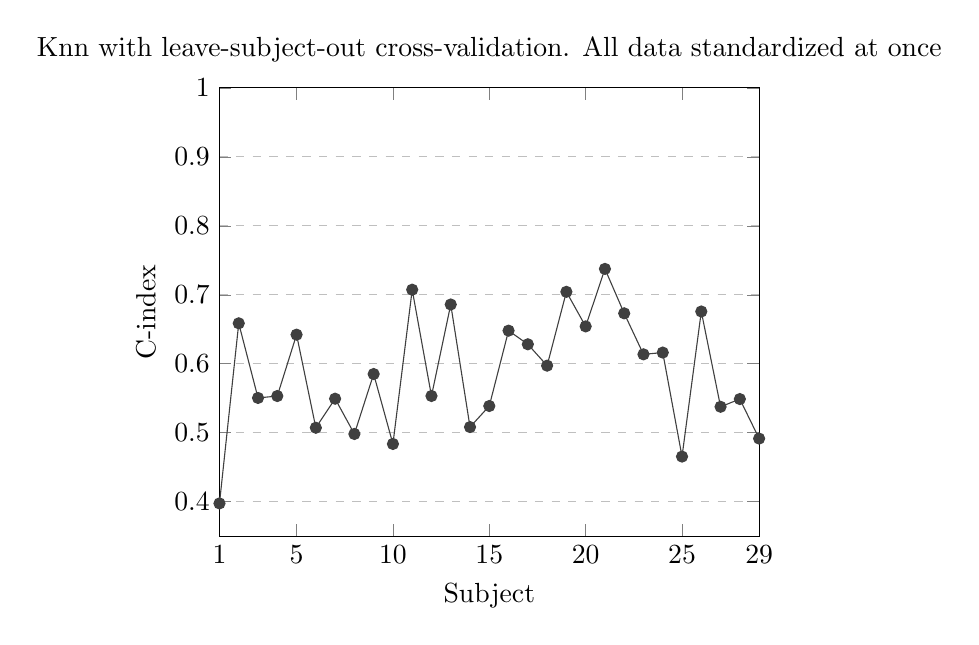
\begin{tikzpicture}
    \begin{axis}[
    title={Knn with leave-subject-out cross-validation. All data standardized at once},
    xlabel={Subject},
    ylabel={C-index},
    xmin=1, xmax=29,
    ymin=0.35, ymax=1,
    xtick={1, 5, 10, 15, 20, 25, 29},
    ytick={0.4, 0.5, 0.6, 0.7, 0.8, 0.9, 1.0},
    legend pos=north west,
    ymajorgrids=true,
    grid style=dashed,
    ]
    \addplot[color=darkgray, mark=*]
      coordinates {
        (1,0.39751117606602476)
        (2,0.6586539610705209)
        (3,0.5504238229197512)
        (4,0.5531962503779861)
        (5,0.6421828229334562)
        (6,0.5071908550243299)
        (7,0.5493156448778556)
        (8,0.4981873111782477)
        (9,0.5851190476190476)
        (10,0.4837078651685393)
        (11,0.707379560011139)
        (12,0.553274494755692)
        (13,0.6859379329454143)
        (14,0.508215206185567)
        (15,0.5387321160382579)
        (16,0.6479975112913633)
        (17,0.6282311244398249)
        (18,0.5972347122302158)
        (19,0.704277656782264)
        (20,0.654164530071057)
        (21,0.7375350982751705)
        (22,0.6731036882393876)
        (23,0.6136530283032703)
        (24,0.6162162162162163)
        (25,0.4654261428899609)
        (26,0.675770248357088)
        (27,0.5376172568241359)
        (28,0.5488139825218477)
        (29,0.4915267037216046)
      };
    \end{axis}
  \end{tikzpicture}
\end{center}

\begin{center}
  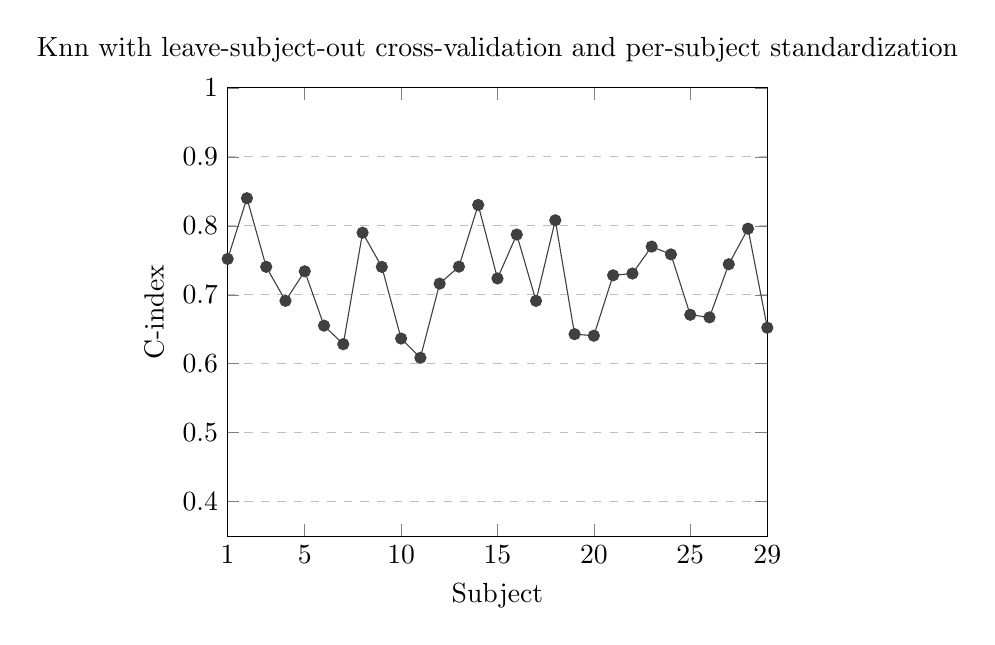
\begin{tikzpicture}
    \begin{axis}[
        title={Knn with leave-subject-out cross-validation and per-subject standardization},
        xlabel={Subject},
        ylabel={C-index},
        xmin=1, xmax=29,
        ymin=0.35, ymax=1,
        xtick={1, 5, 10, 15, 20, 25, 29},
        ytick={ 0.4, 0.5, 0.6, 0.7, 0.8, 0.9, 1.0},
        legend pos=north west,
        ymajorgrids=true,
        grid style=dashed,
    ]
    \addplot[color=darkgray, mark=*]
        coordinates {
          (1,0.7519987964236589)
          (2,0.8400313921710794)
          (3,0.7405380145099201)
          (4,0.6912488660417296)
          (5,0.7340317752705503)
          (6,0.6552483200741485)
          (7,0.6283877434843947)
          (8,0.7899546827794562)
          (9,0.740424430641822)
          (10,0.6365037888685654)
          (11,0.6087023113338903)
          (12,0.7161678178562292)
          (13,0.7407869215849265)
          (14,0.830290664375716)
          (15,0.7237240797828893)
          (16,0.7873075859526224)
          (17,0.6911837374546322)
          (18,0.808041067146283)
          (19,0.6429119897246887)
          (20,0.6406197348179621)
          (21,0.7282290413156839)
          (22,0.7308194154488518)
          (23,0.7698526176858776)
          (24,0.7585684585684586)
          (25,0.6710027567195038)
          (26,0.6672783135614918)
          (27,0.7442639229274064)
          (28,0.795880149812734)
          (29,0.6522021507974867)
     	};
    \end{axis}
  \end{tikzpicture}

\end{center}



\begin{center}
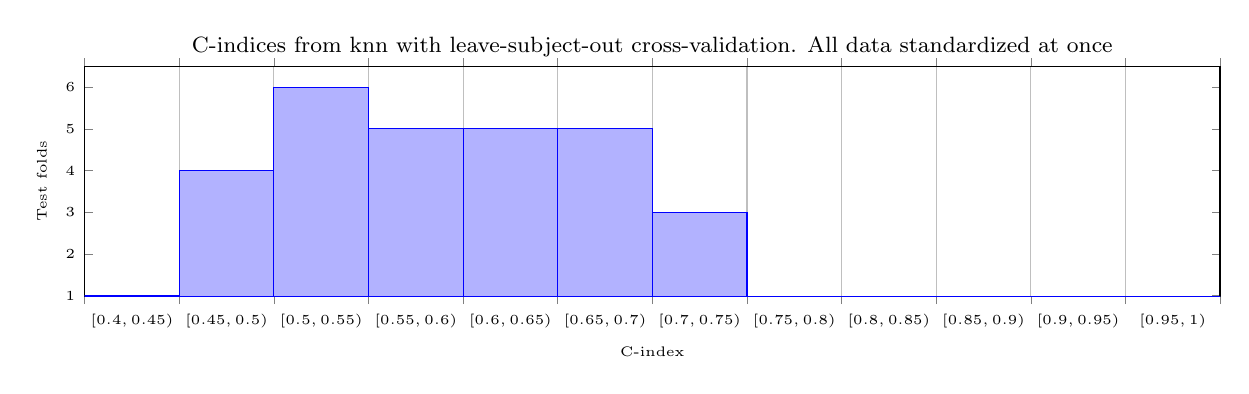
\begin{tikzpicture} \begin{axis}[         
		title={C-indices from knn with leave-subject-out cross-validation. All data standardized at once},
        xlabel={C-index},
        ylabel={Test folds},
        ymin=0.99,
        xmin=0.4, xmax=1.0,
        ybar interval,
        tiny, height=4.5cm,width=16cm, ybar interval,
 		xticklabel= 
        {$[\pgfmathprintnumber\tick,%
        	\pgfmathprintnumber\nexttick)$}] 
\addplot+[hist={bins=12}] coordinates {
(1,0.39751117606602476)
	(2,0.6586539610705209)
	(3,0.5504238229197512)
	(4,0.5531962503779861)
	(5,0.6421828229334562)
	(6,0.5071908550243299)
	(7,0.5493156448778556)
	(8,0.4981873111782477)
	(9,0.5851190476190476)
	(10,0.4837078651685393)
	(11,0.707379560011139)
	(12,0.553274494755692)
	(13,0.6859379329454143)
	(14,0.508215206185567)
	(15,0.5387321160382579)
	(16,0.6479975112913633)
	(17,0.6282311244398249)
	(18,0.5972347122302158)
	(19,0.704277656782264)
	(20,0.654164530071057)
	(21,0.7375350982751705)
	(22,0.6731036882393876)
	(23,0.6136530283032703)
	(24,0.6162162162162163)
	(25,0.4654261428899609)
	(26,0.675770248357088)
	(27,0.5376172568241359)
	(28,0.5488139825218477)
	(29,0.4915267037216046)

    }; 
\end{axis} 
\end{tikzpicture}
\end{center}




\begin{center}
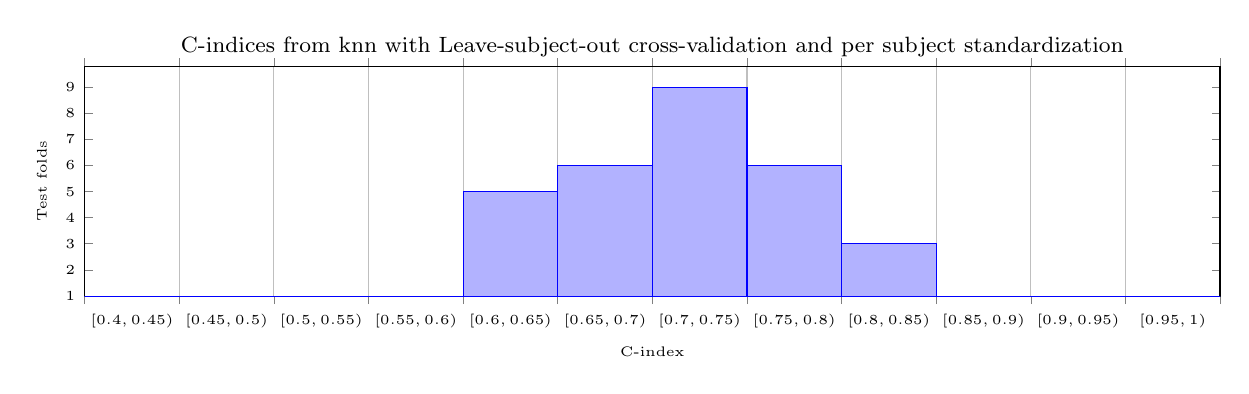
\begin{tikzpicture} \begin{axis}[         
		title={C-indices from knn with Leave-subject-out cross-validation and per subject standardization},
        xlabel={C-index},
        ylabel={Test folds},
        ymin=0.99,
        xmin=0.4, xmax=1.0,
        ybar interval,
        tiny, height=4.5cm,width=16cm, ybar interval,
 		xticklabel= 
        {$[\pgfmathprintnumber\tick,%
        	\pgfmathprintnumber\nexttick)$}] 
\addplot+[hist={bins=12}] coordinates {
    (1,0.7519987964236589)
    (2,0.8400313921710794)
    (3,0.7405380145099201)
    (4,0.6912488660417296)
    (5,0.7340317752705503)
    (6,0.6552483200741485)
    (7,0.6283877434843947)
    (8,0.7899546827794562)
    (9,0.740424430641822)
    (10,0.6365037888685654)
    (11,0.6087023113338903)
    (12,0.7161678178562292)
    (13,0.7407869215849265)
    (14,0.830290664375716)
    (15,0.7237240797828893)
    (16,0.7873075859526224)
    (17,0.6911837374546322)
    (18,0.808041067146283)
    (19,0.6429119897246887)
    (20,0.6406197348179621)
    (21,0.7282290413156839)
    (22,0.7308194154488518)
    (23,0.7698526176858776)
    (24,0.7585684585684586)
    (25,0.6710027567195038)
    (26,0.6672783135614918)
    (27,0.7442639229274064)
    (28,0.795880149812734)
    (29,0.6522021507974867)}; 
\end{axis} 
\end{tikzpicture}
\end{center}


\section{Source code}
Below is listed the source code of the program. For syntax highlighting, please visit my \href{https://github.com/jootimo/ml_repo}{GitHub page}. File $\href{https://github.com/jootimo/ml_repo/blob/master/pain_analysis.py}{pain\_analysis.py}$ handles the parsing of the data file, standardization, cross-validations, calling the knn-utilities and the C-index computations. $\href{https://github.com/jootimo/ml_repo/blob/master/knn.py}{knn.py}$ was written for the previous exercises and contains utilities for the k nearest neighbors algorithm.\\

I used some external libraries:
\begin{itemize}
\item \emph{math} for square root
\item \emph{operator} for sorting a list on values of one index
\item \emph{partial} for function argument binding
\item \emph{ndarray} for transforming an array into a list
\item \emph{stats} for z-score standardization
\end{itemize}

\vspace*{1cm}

\renewcommand{\sfdefault}{pcr}
\fontfamily{pcr}\selectfont

\textbf{pain\_analysis.py:}\\
\footnotesize
\begin{lstlisting}
import knn                      # K-nearest-neighbors utilities
from functools import partial   # Function argument binding
from numpy import ndarray       # array -> list conversion
from scipy import stats         # z-score

DATA_FILENAME = "data/painsignals.csv"

IX_SUBJECT      = 0
IX_TEST         = 1
IX_MEAS_ID      = 2
IX_HR           = 3
IX_RRPM         = 4
IX_GSR          = 5
IX_RMSCORR      = 6
IX_RMSORB       = 7
IX_LABEL        = 8

NUM_NUMERIC_FEATURES = 5

# Open file with name filename and parse comma separated values a into 2-d list
#
# @param    filename
def open_and_parse(filename):
    data = []

    with open(filename, "r") as filestream:

        for line in iter(filestream.readline, ''):
            line = list(line.split(','))

            #First row is headers, skip it
            if line[0] == "subject":
                continue

            #Parse rows into lists
            for i in range(0, len(line)):
                for char in range(0, len(line[i])):

                    #Remove newline characters
                    if type(line[i]) == "str":
                        line[i].replace('\n', '')

                    #Cast to correct type
                    if i in [IX_SUBJECT, IX_MEAS_ID, IX_TEST, IX_LABEL]:
                        line[i] = int(line[i])
                    else:
                        line[i] = float(line[i])

            data.append(line)

    return data

# Get the data that belongs to a single subject 
#
# @param    subject_id  Id of the subject to get data of
# @param    data        2-d data list
#
# @return   Rows in data belonging to subject with id subject_id
def get_rows_of_subject(subject_id, data):
    rows = []
    for row in data:
        if(row[IX_SUBJECT] == subject_id):
            rows.append(row)

    return rows

# Get the data that belongs to other subjects than the specified subject
#
# @param    subject_id  The subject NOT to get data of
# @param    data        2-d data list
#
# @return   Rows in data that don't belong to subject with id subject_id
def get_rows_of_other_subjects(subject_id, data):
    rows = []
    for row in data:
        if(row[IX_SUBJECT] != subject_id):
            rows.append(row)

    return rows

# Get the ids of subjects in data
#
# @param    data    2-d data list
#
# @reuturn  List of subject ids in data  
def get_subject_ids(data):
    subject_ids = []
    prev_id = -1
    for row in data:
        current_id = row[IX_SUBJECT]
        if current_id != prev_id:
            subject_ids.append(int(current_id))
            prev_id = current_id

    return subject_ids


# Get the values of hr, rrpm, gsr, rmscorr, rmsorb from data
#
# @param    data    2-d data list
#
# @return   2-d list containing only the feature values
def get_features(data):
    features = []
    for row in data:
        features.append(row[IX_HR : IX_RMSORB + 1])

    return features

# Get the pain labels from data
#
# @param    data    2-d data list
#
# @return   2-d list containing only the label values
def get_labels(data):
    labels = []
    for row in data:
        labels.append(row[IX_LABEL])

    return labels


# Standardize a list with z-score
# 
# @param    data    The list to standardize
#
# @return   The standardized data
def z_score_list(data):
    standardized = ndarray.tolist(stats.zscore(data.copy()))
    return standardized


# Standardize the features of each subject independently
#
# @param    data                2-d data list
# @param    ix_features_start   Index in data where the features start
# @param    num_features        Number of features in data
# @param    f_standardize       Function to standardize with
#
# @return   Per-subject standardized data
def standardize_features_per_subject(data, ix_features_start, num_features, f_standardize):
    data_standardized = []
    subject_ids = get_subject_ids(data)

    for id in subject_ids:
        rows = get_rows_of_subject(id, data)
        features = get_features(rows)
        
        #Standardize rows of this subject
        features_standardized = f_standardize(features)

        for row_ix in range(0, len(rows)):
            #Place the standardized values to the correct place 
            #in the row 
            row_concat = rows[row_ix][0:ix_features_start]

            for feat in features_standardized[row_ix]:
                row_concat.append(feat)

            row_concat = (row_concat 
                + rows[row_ix][ix_features_start + num_features : len(rows[row_ix])])

            data_standardized.append(row_concat)

    return data_standardized


# Standardize the data
#
# @param    data                2-d data list
# @param    ix_features_start   Index in data where the features start
# @param    num_features        Number of features in data
# @param    f_standardize       Function to standardize with
#
# @return   Standardized data
def standardize_features(data, ix_features_start, num_features, f_standardize):
    data_standardized = []

    features = get_features(data)
    features_standardized = f_standardize(features)

    for row_ix in range(0, len(data)):
        #Place the standardized values to the correct place 
        #in the row 
        row_concat = data[row_ix][0:ix_features_start]

        for feat in features_standardized[row_ix]:
            row_concat.append(feat)

        row_concat = (row_concat 
            + data[row_ix][ix_features_start + num_features : len(data[row_ix])])
        data_standardized.append(row_concat)

    return data_standardized


# Perform k-fold cross-validation where each fold contains only data from
# a single subject
#
# @param    data_matrix     2-d data list 
# @param    num_neighbors   The number of neighbors used in knn
# @param    f_standardize   Function used for standardizing the data
def cross_validate_per_subject(data_matrix, f_standardize, f_predict):

    data = standardize_features_per_subject(
        data_matrix, IX_HR, NUM_NUMERIC_FEATURES, f_standardize)

    subject_ids = get_subject_ids(data)

    c_ixs = []

    for subj_id in subject_ids:
        test_data = get_rows_of_subject(subj_id, data)
        training_data = get_rows_of_other_subjects(subj_id, data)

        c_ixs.append(f_predict(test_data, training_data, subj_id))

    print("Average C-index: " + str(sum(c_ixs) / float(len(c_ixs))))


# Perform k-nearest-neighbors classification for test data
# and get the c-index
#
# @param    test_data       Data to predict labels of
# @param    trainining_data Data to calculate neighbors from
# @param    subject_id      Id of the subject the test data belongs to. Only used for printing
# @param    k               The number of neighbors to search
#
# @return   c-index for predictions
def knn_classification_and_c_index(test_data, training_data, subject_id, k):
    test_labels = get_labels(test_data)
    training_labels = get_labels(training_data)

    test_features = get_features(test_data)
    training_features = get_features(training_data)

    # Get nearest neighbors for every object in test set
    neighbors = knn.compute_nearest_neighbors(test_features, training_features, k)

    predictions = []
    actuals = []
    for measurement in range(0, len(neighbors)):
        prediction = knn.majority_class(neighbors[measurement], training_labels)
        actual = test_labels[measurement]

        predictions.append(prediction)
        actuals.append(actual)

    c_ix = knn.c_index(actuals, predictions)
    print("(" + str(subject_id) + "," + str(c_ix) + ")")

    return(c_ix)


####################################
########## Actual script ###########
####################################

DATA = open_and_parse(DATA_FILENAME)

#Bind the argument 'k' to function knn_classification_and_c_index
NUM_NEIGHBORS = 37
F_PREDICT = partial(knn_classification_and_c_index, k=NUM_NEIGHBORS)

cross_validate_per_subject(DATA, z_score_list, F_PREDICT)

\end{lstlisting}

\vspace*{1cm}
\normalsize
\textbf{knn.py:}\\
\footnotesize
\begin{lstlisting}
from math import sqrt
from operator import itemgetter

# Calculate the Euclidean distance between data points a and b
#
# @param    a   list of attribute values
# @param    b   list of attribute values
#
# @return   distance between a and b or -1 if lists have different lenghts 
def distance(a, b):
    len_a = len(a)
    len_b = len(b)

    if len_a != len_b:
        return(-1)
    else:
        dist = 0
        for i in range(0, len_a):
            dist += (a[i] - b[i]) ** 2

        return sqrt(dist)


# Compute distances from each data point in training data to that in test data
#
# @param    training_data  list of numerical data rows, excluding the attribute to predict
# @param    test_data      list of the data object to calculate distances to
#
# @return   distance list
def compute_distances(test_data, training_data):

    distances = []
    
    for i in range(0, len(test_data)):
        row = []
        for j in range(0, len(training_data)):
            dist = distance(test_data[i], training_data[j])
            row.append(dist)

        distances.append(row)

    return(distances)

# Compute nearest neighbors of the given data object
#
# @param    test_data       data object to compute distances to
# @param    training_data   data that the distances are computed to
# @param    num_neighbors   value of k
#
# @return   Indices of num_neighbors nearest neighbors of test_data in training_data
def compute_nearest_neighbors(test_data, training_data, num_neighbors):
    #Compute distances to test_data
    distances = compute_distances(test_data, training_data)
    neighbors = []
    for ix_test_obj in range(0, len(test_data)):
        #Iterate over the distance list and create list of (row index, distance) pairs
        ixs_and_distances = []
        for i in range(0, len(distances[ix_test_obj])):
            ixs_and_distances.append([ i, distances[ix_test_obj][i] ])

        #Sort the list on distances and include only first num_neighbors elements
        ixs_and_distances.sort(key = itemgetter(1))
        k_nearest = ixs_and_distances[0 : num_neighbors]

        #Only return neighbor indices in training_data
        neighbors_of_row = []
        for n in k_nearest:
            neighbors_of_row.append(n[0])

        neighbors.append(neighbors_of_row)

    return(neighbors)


# Get the majority class in list neighbors
#
# @param    neighbor_ixs   list of neighbor indices
# @param    classes        list of the correct classes in the training data
#
# @return   value of the majority class 
def majority_class(neighbor_ixs, classes):
    neighbor_classes = []
    for n in neighbor_ixs:
        neighbor_classes.append(classes[n])
    
    return(max(set(neighbor_classes), key = neighbor_classes.count))
\end{lstlisting}


\end{document}